\question
Вася приехал в Санкт-Петербург, и чтобы прокормить себя устроился на работу таксистом. Однажды утром Васе поступил заказ: отвезти преподавателя Антона Сергеевича в ИТМО, чтобы провести первую пару. Антон Сергеевич пообещал Васе, что даст ему 5000₽ на чай, если тот приедет как можно скорее (за минимально возможное время). Помогите Васе решить задачу и заработать на обед.

На карте необходимо попасть из точки A в точку B за минимально возможное время. Красным обозначено количество минут, которое требуется на то, чтобы проехать от одного перекрёстка к другому. В ответе укажите полученное наименьшее время, и схематически изобразите самый быстрый путь:

\begin{minipage}[h]{0.45\linewidth}
\center{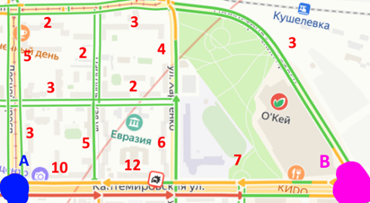
\includegraphics[width=0.7\textwidth]{pic/73.png} }
\end{minipage}

---------------

Автор -- Тимур Гонтарь
